\documentclass[12pt, a4paper]{article}
\usepackage[left=2.54cm, right=2.54cm, bottom=2.54cm, top=2.54cm]{geometry}
\linespread{1}
\usepackage{setspace}
\usepackage[utf8]{inputenc}
\usepackage{blindtext}
\usepackage[T1]{fontenc}
\usepackage{xcolor}
\usepackage{amsfonts}
\usepackage{amsmath}
\usepackage{amssymb}
\usepackage{fancyhdr}
\pagestyle{fancy}
\fancyhead{}
\fancyfoot{}
\fancyfoot[R]{\thepage}
\renewcommand{\headrulewidth}{2pt}
\renewcommand{\footrulewidth}{2pt}
\usepackage{graphicx}
\usepackage{multicol}
\usepackage{tikz}
\usetikzlibrary{arrows}

\title{Latihan ETS}
\author{Riyannizaar Dwi Amarullah \\ 5025241121}
\date{October 2024}

\begin{document}

\maketitle

\begin{enumerate}
    \item Diberikan suatu fungsi $f(x) = 2 + \sqrt{x-1}$ dan garis $l$ yang melalui titik $(1,2)$ dan $(7,5)$.
    \begin{enumerate}
        \item Sketsa kurva $f(x)$ dan garis $l$. \\
        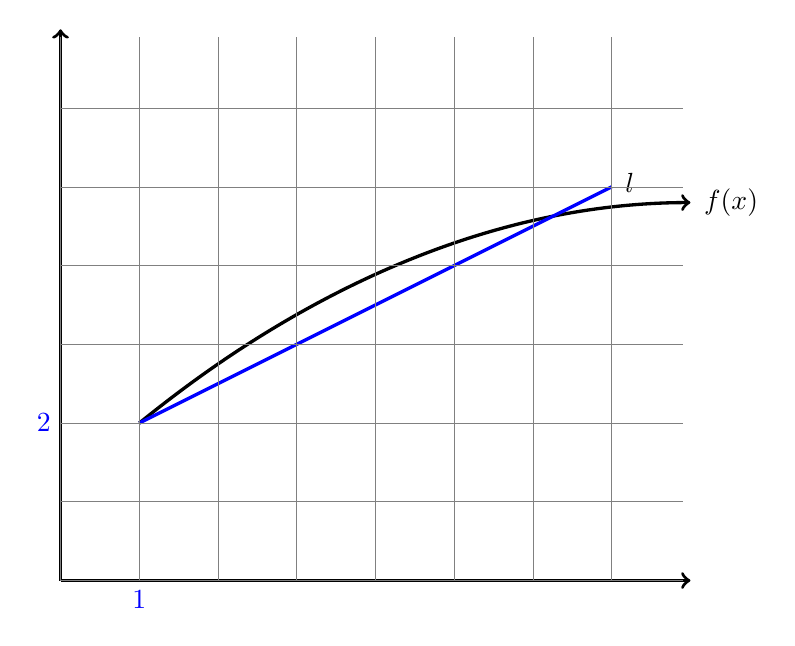
\begin{tikzpicture}
            \draw [black, ->, very thick] (0,0) -- (8,0);
            \draw [black, ->, very thick] (0,0) -- (0,7);
            \draw [black, <-, very thick] (8,4.8) parabola (1,2);
            \draw [blue, very thick] (1,2) -- (7,5);
            \draw[fill=black] (8.05,4.8) circle (0pt) node[right] {$f(x)$};
            \draw[fill=black] (7.05,5.05) circle (0pt) node[right] {$l$};
             \foreach \x in {1} 
            \draw[shift={(\x,0)}, color=blue] node[below] {$1$};
             \foreach \y in {2} 
            \draw[shift={(0,\y)}, color=blue] node[left] {$2$};
            \draw[step=1cm,gray,very thin] (0,0) grid (7.9,6.9);
        \end{tikzpicture}

        \item Titik potong antara kurva $f(x)$ dan garis $l$ \\
        $\bullet$ Tipot $x, y = 1$ \\
        $1 = 2 + \sqrt{x-1}$ \\
        $-1 = \sqrt{x-1}$ \\
        $1 = x-1$ \\
        $2 = x$ \\
        $x = 2$ (2,0) \\

        $\bullet$ Tipot $y, x = 1$ \\
        $y = 2 + \sqrt{1-1}$ \\
        $y = 2$ (0,1) \\

        Jadi garis $l$ memotong $f(x)$ di titik (1,2) 
    \end{enumerate}
    \item Diberikan fungsi $f(x) = a + \sqrt{x-b}$ dan $g(x) = (x-a)^2 + b$ \\
    \begin{enumerate}
        \item Domain dan range f(x) \\
        Domain $\Rightarrow$ Nilai di dalam akar tidak boleh negatif \\
        $x-b \geq 0$ \\
        $\Leftrightarrow x \geq b$ \\
        $D(f) = \{x \geq b, x \in \mathbb{R}\}$ \\
        $R(f) = \{x \geq a, x \in \mathbb{R}\}$ 
        \item Domain $g(x)$ agar fungsi $f(x)$ dan $g(x)$ saling invers \\
        $g(x) = (x-a)^2 + b$ \\
        $D(g) = \{x \geq a, x \in \mathbb{R}\}$ \\
        $R(g) = \{x \geq b, x \in \mathbb{R}\}$ 
        \item Sketsa kurva $f(x)$ dan $f^{-1}(x)$, $(a = 2, b = 1)$ \\
        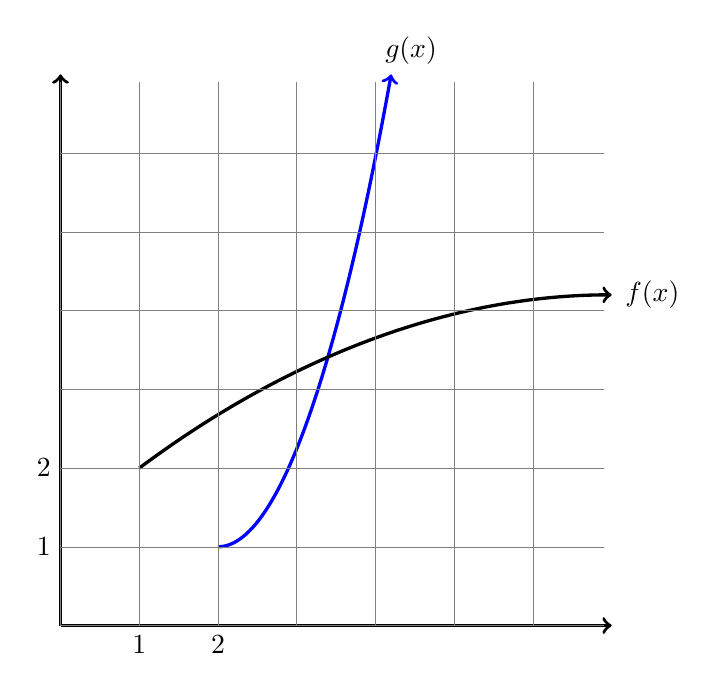
\begin{tikzpicture}
            \draw [black, ->, very thick] (0,0) -- (7,0);
            \draw [black, ->, very thick] (0,0) -- (0,7);
            \draw [blue, ->, very thick] (2,1) parabola (4.2,7);
            \draw [black, <-, very thick] (7,4.2) parabola (1,2);
            \draw[fill=black] (7.05,4.2) circle (0pt) node[right] {$f(x)$};
            \draw[fill=black] (4,7.3) circle (0pt) node[right] {$g(x)$};
             \foreach \x in {1, 2} 
            \draw[shift={(\x,0)}, color=black] node[below] {$\x$};
             \foreach \y in {1, 2} 
            \draw[shift={(0,\y)}, color=black] node[left] {$\y$};
            \draw[step=1cm,gray,very thin] (0,0) grid (6.9,6.9);
        \end{tikzpicture}
    \end{enumerate}
    \item $g(x)$ =  $\left\{ \begin{array}{rcl}
        (px)^2 & \mbox{,} & x \leq 2 \\ 
        (x+p) & \mbox{,} & x > 2 \\
        \end{array}\right.$ \\
    $\bullet$ Nilai $p$ yang mungkin agar $g(x)$ kontinu \\
    lim$_{x\rightarrow2^-} g(x) =$  lim$_{x\rightarrow2^+} g(x)$ \\
    $\Leftrightarrow$ lim$_{x\rightarrow2^-} (px)^2$ =  lim$_{x\rightarrow2^+} (x+p)$ \\
    $\Leftrightarrow (2p)^2 = 2 + p$  \\
    $\Leftrightarrow 4p^2 - p -2 = 0$  \\
    Jadi $p = \frac{1 \pm \sqrt{33}}{8}$ \\
    Jadi, agar $g(x)$ kontinu, nilai $p = \frac{1 + \sqrt{33}}{8}$ atau $p = \frac{1 - \sqrt{33}}{8}$
    \item Tentukan semua nilai $x$ yang memenuhi $|2x-1| + x = |x-2| + 3$ \\
        $|2x-1|$ =  $\left\{ \begin{array}{rcl}
        2x-1 & \mbox{,} & x \geq -\frac{1}{2} \\ 
        -2x+1 & \mbox{,} & x < -\frac{1}{2} \\
        \end{array}\right.$
        $|x-2|$ =  $\left\{ \begin{array}{rcl}
        x-2 & \mbox{,} & x \geq 2 \\ 
        -x+2 & \mbox{,} & x < 2 \\
        \end{array}\right.$ \\

    $\bullet$ untuk $x < -\frac{1}{2}$ \\
    $-2x-1+x = (-x+2) + 3$ \\
    $\Leftrightarrow -x-1 = -x+5$ \\
    $\Leftrightarrow 0 = 6$ (Tidak memenuhi)\\
    $\bullet$ untuk $-\frac{1}{2} \leq x < 2$ \\
    $2x+1+x = (-x+2) + 3$ \\
    $\Leftrightarrow 3x+1= -x + 5$ \\
    $\Leftrightarrow 4x= 4$ \\
    $\Leftrightarrow x= 1$ \\ 
    $\bullet$ untuk $x \geq 2$ \\ 
    $2x+1+x = (x-2)+3$ \\
    $\Leftrightarrow 3x+1= x+1$ \\ 
    $\Leftrightarrow 2x= 0$ \\
    $\Leftrightarrow x= 0$ (Tidak memenuhi)\\
    Jadi penyelesaiannya adalah $x = 1$ 

    \item $f(x) = \frac{x^3 + x^2 + x - 3}{x-1}$ \\
    lim$_{x\rightarrow1} f(x)$ \\
    = lim$_{x\rightarrow1} \frac{x^3 + x^2 + x - 3}{x-1}$ \\
    = lim$_{x\rightarrow1} \frac{(x-1)(x^2+2x+3)}{x-1}$ \\
    = lim$_{x\rightarrow1} (x^2+2x+3)$ \\
    = 6\\
\end{enumerate}

\end{document}
